\documentclass[5p]{elsarticle}

\usepackage{lineno,hyperref}
\usepackage{amsfonts}
\usepackage{amsmath}
\usepackage{mathtools}

\modulolinenumbers[5]

\journal{Journal of \LaTeX\ Templates}

%%%%%%%%%%%%%%%%%%%%%%%
%% Elsevier bibliography styles
%%%%%%%%%%%%%%%%%%%%%%%
%% To change the style, put a % in front of the second line of the current style and
%% remove the % from the second line of the style you would like to use.
%%%%%%%%%%%%%%%%%%%%%%%

%% Numbered
%\bibliographystyle{model1-num-names}

%% Numbered without titles
%\bibliographystyle{model1a-num-names}

%% Harvard
%\bibliographystyle{model2-names.bst}\biboptions{authoryear}

%% Vancouver numbered
%\usepackage{numcompress}\bibliographystyle{model3-num-names}

%% Vancouver name/year
%\usepackage{numcompress}\bibliographystyle{model4-names}\biboptions{authoryear}

%% APA style
%\bibliographystyle{model5-names}\biboptions{authoryear}

%% AMA style
%\usepackage{numcompress}\bibliographystyle{model6-num-names}

%% `Elsevier LaTeX' style
\bibliographystyle{elsarticle-num}
%%%%%%%%%%%%%%%%%%%%%%%



\begin{document}

\begin{frontmatter}

\title{Obscured by the cloud: A resource allocation framework to model cloud outage events\tnoteref{mytitlenote}}
%%\tnotetext[mytitlenote]{}

%% Group authors per affiliation:
%% \author{Elsevier\fnref{myfootnote}}
%% \address{Radarweg 29, Amsterdam}
%% \fntext[myfootnote]{Since 1880.}

%% or include affiliations in footnotes:
\author[mymainaddress]{Jonathan Dunne\corref{mycorrespondingauthor}}
\cortext[mycorrespondingauthor]{Corresponding author}
\ead{jonathan.dunne.2015@mumail.ie}

\author[mymainaddress]{David Malone}
%%\ead[url]{www.elsevier.com}

\address[mymainaddress]{Hamilton Institute, Maynooth University, Kildare, Ireland}

\begin{abstract}
As SME's adopt cloud technologies and rapid delivery models as a means to provide high value customer offers, there is a clear focus on uptime. Cloud outages represent a challenge to an SME's to deliver and maintain a services platform. If a Cloud platform suffers from downtime this can have a negative effect on business revenue. Additionally outages can divert resources from product development/delivery tasks to reactive remediation. These challenges are more immediate to SME's or micro teams with a small pool of resources at their disposal. Therefore it is necessary to develop a framework which can be used to model the arrival of cloud outage events. A framework which can be used by Cloud operations teams to manage their scarce pool of resources to resolve outages, thereby minimising impact to service delivery. This article considers existing modelling techniques such as the M/M/1 queue, and proposes a more accurate approach. We first calculate the inter arrival and service distributions. Next we formally test for dependence between event arrivals. We then model a series of outage events in a G/G/1 queue with a Monte Carlo simulation to determine queue busy time.  Finally we compare the precision of our framework against an M/M/1 simulation and observed outage event data. The results of this study demonstrate that this framework can improve the estimation of Cloud outage events and aid DevOps resource planning.
\end{abstract}

\begin{keyword}
Outage simulation \sep Resource allocation model \sep Queuing Theory 
\end{keyword}

\end{frontmatter}

\linenumbers

\section{Introduction}
Cloud outage prediction and resolution is an important activity in the management of a cloud service. Recent media reports have documented cases of cloud outages from high profile cloud service providers \cite{CRN2016outage}. During 2016 alone the CRN website has documented ten highest profile cloud outages to have occurred so far.  Due to the increasing complex nature of the data centre infrastructure coupled with the rapid continuous delivery of incremental software updates it seems that cloud outages are with us for the time being.

For operations teams that maintain a cloud infrastructure, they rely on state of the art monitoring and alert systems to determine when an outage occurs. Examples of monitoring solutions include: New Relic, IBM Predictive Insights and Ruxit. Once a new outage is observed, depending on the outage type (e.g. Software component, infrastructure, hardware etc) additional relevant experts may be called to remediate the issue. The time taken to resolve the issue may depend on a number of factors: ability to find the relevant expert, swift problem diagnosis and velocity of the pushing a fix to production systems. 

Both SME's and micro teams within large organisation's face a number of challenges when adopting a cloud platform and a mechanism to deliver products and services. A number of recent studies have outlined that both frequency and duration of outage events are key challenges. Almost all European SME's (93\%) employ less than ten people \cite{europa2015sme}. Ensuring that adequate skills and resources are available to accommodate incoming outage events is highly desirable.

Downtime is bad for business. Whether a company provides a hosting platform, more commonly known as Platform as a Service (PaaS) or for a company that consumes such a platform to deliver their own services, more commonly known as Software as a Service (SaaS). The end result is the same: Business disruption, lost revenue, recovery/remediation costs etc. A recent US study which looked at the cost of data centre downtimes, calculated the mean cost to be \$5617 per minute of downtime \cite{DCcost}.

In preparation for this study, a thorough search of current literature was conducted. No frameworks to model cloud outage events were found. This study observed that outage events arrive over a period of time, which require fixing to return a system to a steady state. With these attributes in mind, our literature search focuses on  
queuing theory and distribution fitting for repairable systems.

Another consideration is the idea of event dependence. Typical off the shelf single-server queue models such as M/M/1 and G/G/1 assume that the inter-arrival and service times between events are independent \cite{MM1}. However if some form of dependence is found between events how useful would a queuing model which assumes independence compare against that of a queuing model with dependence properties.

In this paper we propose a framework that a micro team or SME can leverage to best manage their existing resource pool. The core idea of this framework is for operations teams to use a special case of the G/G/1 queue to model the inter-arrival and service times of outage events. Our study shows that the special case of G/G/1 delivers a high degree of accuracy compared to off the shelf queuing models like M/M/1. Additionally our framework also considers dependence between overlapping outage events. This article consists of a study of outage event data from a large enterprise dataset. By analysis of outage event data this study shows the efficacy of the G/G/1 special case and how it can be used to reasonably model cloud outage event data. Additionally we highlight the shortcomings of the M/M/1 queue specifically in the realm of service times of repairable systems, such as cloud based platforms. Finally this study highlights how dependence overlapping between cloud outage's plays a role in the frameworks precision.

To help researchers reproduce and extend the work conducted as part of this study, pseudo-code of the queue modelling framework is provided . By utilising this queue framework, researches will have the ability to test their preferred case of the G/G/1 model against the M/M/1 model.

Further motivation is driven by recent reports and studies into the adoption of Cloud computing.  Carcary et al. \cite{carcary2014adoption} conducted a study into Cloud Computing adoption by Irish SMEs. The key findings of the study were as follows: Almost half the 95 SMEs surveyed had not migrated their services to the cloud. Of those SMEs that had migrated they had not assessed their readiness to adopt cloud computing. Finally the study noted that the main constraints for SMEs adoption of Cloud computing were: Security/compliance concerns, lack of IT skills and data protection concerns. Gholami et al. \cite{gholami2016cloud} provided a detailed review of current cloud migration processes. One of the main migration concerns mentioned was the unpredictability of a cloud environment. Factors that led to this unpredictability included: Network outages and middleware failures. The study concluded that a fixed migration approach is not possible to cover all migration scenarios due to architecture heterogeneity.

The rest of this article is divided up into the following sections: Section 2 introduces background and related work. Section 3 discusses the data set collected (and associated study terminology), outlines the research questions that are answered by this study and the limitations of the dataset. Section 4 outlines the experimental approach and associated results. Section 5 discusses the results of our experiments. Finally in Section 6, we conclude this paper and discuss future work.

\section{Background and related work}

The following section provides some background information on two common cloud services: SaaS and PaaS. Followed by a section on high profile cloud outages that have made the media headlines. Finally this section concludes with a in-depth look at related studies in the field of repairable systems modelling, queuing theory and cloud outage studies.

\subsection{Software as a Service}
SaaS is defined as a delivery and licensing model in which software is used on a subscription basis (e.g. monthly, quarterly or yearly) and where applications or services are hosted centrally \cite{cloudbook2015}. The key benefits for software vendors are the ability for software to be available on a continuous basis (on-demand) and for a single deployment pattern to be used. It is this single deployment pattern that can greatly reduce code validation times in pre-release testing, due to the homogeneous architecture. Central hosting also allows for rapid release of new features and updates through automated delivery processes \cite{datacentre2015}. 

SaaS is now ubiquitous, while initially adopted by large software vendors (e.g. Amazon, Microsoft, IBM, Google and Salesforce) many SMEs are now using the cloud as their delivery platform and licensing model of choice \cite{CRN2015providers}. 

\subsection{Platform as a Service}
PaaS is defined as a delivery and platform management model. This model allows customers to develop and maintain cloud based software and services without the need of building and managing a complex cloud based infrastructure.

The main attraction of PaaS is that it allows SME's to rapidly develop and deliver cloud based software and services. While focusing on their core products and services SMEs are less distracted by having to design, build and service a large complex cloud based infrastructure. 

However one drawback of PaaS is that an SME may not have a full view of the wider infrastructure. Therefore if an outage event occurs at an infrastructure level (e.g. Network, Loadbalancer) an SME may be unaware of the problem until the problem is reported by a customer.

Many companies now offer PaaS as their core service. Once seen as the preserve of a large organisation (e.g. Amazon EC2, Google Apps and IBM Bluemix) a number of smaller dedicated companies also offer PaaS (e.g. Dokku, OpenShift and Kubernetes) \cite{Paas2016}.


\subsection{High profile cloud outages}
A cloud outage is the amount of time that a service is unavailable to the customer. While the benefits of cloud systems are well known, a key disadvantage is that when a cloud environment becomes unavailable it can take a significant amount of time to diagnose and resolve the problem. During this time the platform can be unavailable for all customers.

One of the first cloud outages to make the headlines in recent times was the Amazon outage in April 2011. In summary, the Amazon cloud experienced an outage that lasted 47 hours, the root cause of the issue was a configuration change made as part of a network upgrade. While this issue would be damaging enough for Amazon alone, a number of consumers of Amazon's cloud platform (Reddit, Foresquare) were also affected. \cite{InfoWorld2015outage} 

Dropbox experienced two widespread outages during 2013 \cite{Talbot013DBoutage, Etherington2013DBoutage}. The first in January, users were unable to connect to the service. It took Dropbox 15 hours to restore a full service. No official explanation as to the nature of the outage was given. The second occurred in May, again users were unable to connect to the service. This outage lasted a mere 90 minutes. Again no official explanation was provided.

While great improvements have been made in relation to redundancy, disaster recovery and ring fencing of critical services, the big players in cloud computing are not immune to outages. As of mid 2016 a number of high profile outages were catalogued by the CRN website. \cite{CRN2016outage} Table I provides a summary. 

\begin {table*}[]
\caption {Summary of high profile Cloud outages in the first half of 2016} 
\begin{flushleft}

\begin{tabular}{l | l | l | p{11.4cm} l} \bf {Company} & \bf {Duration} & \bf {Date} & \bf {Outage Details}  
\\ \hline Office 365 & Several days &  18th Jan & Users reported issues accessing their cloud based mail services. The defect was identified and a software fix was applied. This fix proved unsuccessful, thereafter  a secondary fix was developed and applied which was successful.
\\ \hline Twitter & 8 hours  & 19th Jan & Users experienced general operational problems after an internal software update was applied to the production system with faulty code. It took Twitter 8 hours to debug and remediate the defective code.
\\  \hline Salesforce & 10 hours  &  3rd March &  European Salesforce users had their services disrupted due to a storage problem in their EU Data Centre. After the storage issue was resolved, users reported performance degradation.
\\  \hline Symantec & 24 Hours  &  11th April &  A portal to allow customers to manage their cloud  security services became unavailable. The exact nature of the outage was undisclosed. Symantec were required to restore and configure a database to bring the system back online.
\\ \hline Amazon & 10 hours  & 4th June & Local storms in Australia caused Amazon Web Services to lose power. This resulted in a number of EC2 instances to fail, which affected both SaaS and PaaS customers. 
\\ \hline 

 \end{tabular}
\end{flushleft}
\end{table*}

\subsection{Other related studies}
A number of studies have been conducted in relation to cloud outages. Additionally, research has been carried on the time observed to service problems in repairable systems.  A summary of these studies are discussed below. \par

Yuan et al. \cite{yuan2014simple} performed a comprehensive study of distributed system failures. Their study found that almost all failures could be reproduced on reduced node architecture and that performing tests on error handling code could have prevented the majority of failures. They conclude by discussing the efficacy of their own static code checker as a way to check error-handling routines. \par

Hagen et al. \cite{hagen2012efficient} conducted a study into the root cause of the Amazon cloud outage on April 21st 2011. Their study concluded that a configuration change was made to route traffic from one router to another, while a network upgrade was conducted. The backup router did not have sufficient capacity to handle the required load. They developed a verification technique to detect change conflicts and safety constraints, within a network infrastructure prior to execution. \par

Li et al \cite{li2013cloud} conducted a systematic survey of public Cloud outage events. Their findings generated a  framework, which classified outage root causes. Of the 78 outage events surveyed they found that the most common causes for outages included: System issues i.e. (human error, contention) and power outages being the primary root cause. \par

Sedaghat et al \cite{sedaghat2015hard} modelled correlated failures caused by both network and power failures. As part of the study the authors developed a reliability model and an approximation technique for assessing a services reliability in the presence of correlated failures. \par 

Potharaju and Navendu \cite{potharaju2013network} conducted a similar study in relation to network outages, with focus on categorising intra and inter data centre network failures. Two key findings include: Network redundancy is most effective at inter-datacentre level and interface errors, hardware failures and unexpected reboots dominate root cause determination. \par

Bodik et al \cite{bodik2012surviving} analysed the network communication of a large scale web application. Then proposed a framework which achieves high fault tolerance with reduced bandwidth usage in outage conditions. \par 

Synder et al \cite{snyder2015evaluation} conducted a study on the reliability of cloud based systems.The authors developed an algorithm based on a non-sequential Monte Carlo Simulation to evaluate the reliability of large scale cloud systems. The authors found that by intelligently allocating the correct types of virtual machine instances, overall cloud reliability can be maintained with a high degree of precision. \par

Kenney \cite{kenny1993estimating} proposes a model to estimate the arrival of field defects based on the number of software defects found during in-house testing. The model is based on the Weibull distribution which arises from the assumption that field usage of commercial software increases as a power function of time. If we think of cloud outages as a form of field defect, there is much to consider in this model. \par 

Kleyner and O'Connor \cite{o2011practical} propose an important thesis regarding reliability engineering. While emphasis is placed on measuring reliability for both mechanical and electrical/electronic systems, the authors do broaden their scope to discuss reliability of computer software. One aspect of interest is their discussion of the lognormal distribution and its application in modelling for system reliability with wear out characteristics and for modelling the repair times of maintained systems. \par

Almog \cite{almog1979study} analysed repair data from twenty maintainable electronic systems to validate whether either the lognormal or exponential distribution would be a suitable candidate distribution to model repair times. His results showed that in 67\% of datasets the lognormal distribution was a suitable fit, while the exponential was unsuitable in 62\% all of datasets. \par

Adedigba \cite{adedigba2005statistical} analysed the service times from a help desk call centre. Her study showed that the exponential distribution did not provide a reasonable fit for call centre service times. However a log-normal distribution was a reasonable fit for overall service times. Her study also showed that a phase-type distribution with three phases provided a reasonable fit for service times for specific jobs within the call centre job queue. \par

\section{Data set and research methodology}

Cloud outage studies have been shown to provide an effective way to highlight the distribution of failure events. These studies can be leveraged by enterprises to pre-empt common failure patterns \cite{InfoWorld2015outage}. In this and subsequent sections our study will present a data set and queuing model. The aim of which is to illustrate it's efficacy in modelling cloud outage events.  

The study presented in this paper examines approximately 330 outage events from a large cloud based system. The data was collected over a 18-month period (January 2015 to June 2016) and is comprised of four main components: E-mail, Collaboration, Social and Business Support System (BSS). The systems have been deployed within three data centres and are used by customers globally. The software is developed in Java and runs on Linux.

Product development follows a Continuous delivery (CD) model whereby small amounts of functionality are released to the public on a monthly basis. For each outage event the authors have access to the full outage report. This study focuses on the following aspects of the outage event data: The inter-arrival time between each outage, the time to service each outage event and whether or not overlapping outage events are related.

The following terminology will now be defined to provide clear context. These definitions are referenced from wikipedia as no formal IEEE definitions could be obtained \cite{wikidef}.

\begin{itemize}
 \item Downtime (Outage): The term downtime is used to refer to periods when a system is unavailable. Downtime or outage duration refers to a period of time that a system fails to provide or perform its primary function. 
 \item  Maintenance window: In information technology and systems management, a maintenance window is a period of time designated in advance by the technical staff, during which preventive maintenance that could cause disruption of service may be performed.
 \item Tiger Team: A tiger team is a group of experts assigned to investigate and/or solve technical or systemic problems. 
 \item DevOps: is a practice that highlights the collaboration between software development and infrastructure personnel. DevOps may also refer to a team whos core function is to build, deploy and maintain a cloud infrastructure. 
 \item Queuing theory:Is the study of events that form waiting lines or queues. In queuing theory, a model is constructed so that queue lengths, inter-arrival and service times can be predicted \cite{sundarapandian2009probability}.
\end{itemize}

Prior to outlining our research questions, it is useful to understand why queuing theory could be used to model cloud outages events. Outages happen at a specific point in time. The problem is then diagnosed and serviced by tiger and DevOps teams. These characteristics are very similar to the properties of a queue system (i.e. inter-arrival times, service times and queue length). 

Both micro teams and SMEs have less than ten employees \cite{eusmereport2015}, yet are adopting the cloud as a method to deliver software and services. Given the unpredictability of cloud infrastructure architecture, this study is required to understand whether a micro team / SME has adequate resources to manage future cloud outage events. 

This study aims to answer a number of research questions. First, how are the inter-arrival times of cloud outage events distributed? Second, How are the service times of cloud outage events distributed?  Third, can an effective queuing model be built to effectively simulation outage event traffic? Fourth, are overlapping outage events related or can we treat each event as independent? 

\subsection{Inter-arrival time distribution}

Probability distributions are used in statistics to infer how likely it is for an event to happen. In the case of cloud outage inter-arrival times,  we can analyse the data determine which distribution is the best fit. The location properties of a distribution can then be used to infer the likelihood of an event happening. For distribution fitting, the authors used the R package fitdistrplus \cite{fitdistrplus} to fit various distributions to our dataset. To validate the efficacy of each distributions,  the authors used the R package ADGofTest \cite{ADGoF}. 

\subsection{Service time distribution}

This study has similar motivations for cloud outage service times. Being able to determine a probability distribution that best fits this outage event dataset is a useful exercise. By combining both inter-arrival and service time distributions a queue system can then be built. This queue system can be used to model the arrival and service times of cloud outage events. The approach to distribution fitting and validation, is the same as described in the previous sub-section. 

\subsection{Outage event modelling framework}

Queuing models have been used previously across many sciences to simulate the arrival and service times for a collection of events. Typically observed inter-arrival and service times data is used to derive a suitable fitting distribution. Thereafter the distribution location parameters (i.e. mean, rate, shape, scale etc) are used to simulate queue traffic. Simulation experiments are in practice much larger than the number of observations. The reason for this is to compare whether the results of simulated data compares favourably or not to an observed sample data. 

For this study we look at how a queuing system can be used to model cloud outage events. Our queue system was developed using the C programming language. Our study conducted a number of simulations using different sample sizes (i.e. 10k, 100k \& 1M) against a G/G/1 system based on a suitable sample distributions. Furthermore our study also conducted the same three simulations against an M/M1 queue. 

An assessment of the usefulness of such simulations is given within the context of resource management within a micro team or SME. Can such simulations provide a reasonable degree of precision to aid resource planning of DevOps / Tiger teams with constrained levels of staffing.

\subsection{Assessment for no association and linkage between overlapping outage events}

As discussed earlier, the M/M/1 queuing system assumes that arrivals are independent. This is due to the understanding that both arrival and service times are governed by a Poisson process. For G/G/1 (i.e. non Poisson distribution) queues, there is no such assumption of independence. However, the occurrence of cascading (i.e. dependent) outages events can play a role in the shape of both inter-arrival and service distributions. Therefore for the final part of our research, this study formally tests whether the arrival times of outage events are independent or not. 

The following method will be used: Defect outage reports will be analysed to determine if an arrival overlaps with the service time of a prior outage event. Next the outage reports will be examined to determine if the two overlapping outages are related by component area and root cause. The outage counts will then be arranged in a 2 by 2 contingency table format. Fishers exact test for independence\cite{fisher1922interpretation}\cite{fisher1925statistical} is then conducted. For the actual test the authors used the R library fisher.test \cite{FisherExact}. 

\subsection{Study limitations / Threats to validity}

The dataset has a number of practical limitations, which are now discussed. The event data collected for this study comprised of outage reports from an enterprise system deployed over three data centres. For the purposes of event modelling the authors have assumed a simple queue. In other words a queuing system with one "server". 

Given the lack of studies in the area of modelling cloud outage events within a queuing framework, the authors wanted to validate such a framework in the context of a simple queue initially. 

Finally the outage events that form part of this study are from an enterprise cloud system. The outage events are applicable to the software domain of BSS, Collaboration, Email and social applications. As a consequence the analysis may not be relevant outside of these fields.

\section{Results}
The results of the study are now discussed. This section shall follow the same format as the methodology section.

\subsection{Inter-arrival time distribution}

\begin {table}
\caption {Inter-arrival time distributions :  Goodness of fit summary} 
\begin{center}
\begin{tabular}{p{2.1cm} |  p{3.1cm} | p{1.3cm}} \hline \bf{Distribution} & \bf{AD Test Statistic} & \bf{p-value}
\\ \hline Pareto & 0.95 & 0.3836 
\\ loglogistic & 1.93 & 0.10
\\ lognormal & 3.79 & 0.01
\\ gamma & 632.89 & 1.83e-06	
\\ exponential & Infinity  & 1.83e-06
\\ logistic & Infinity & 1.83e-06	
\\ weibull  & Infinity & 1.83e-06 
\\ \hline
\end{tabular}
\end{center}
\end{table}

\begin{figure*}[]
\begin{center}
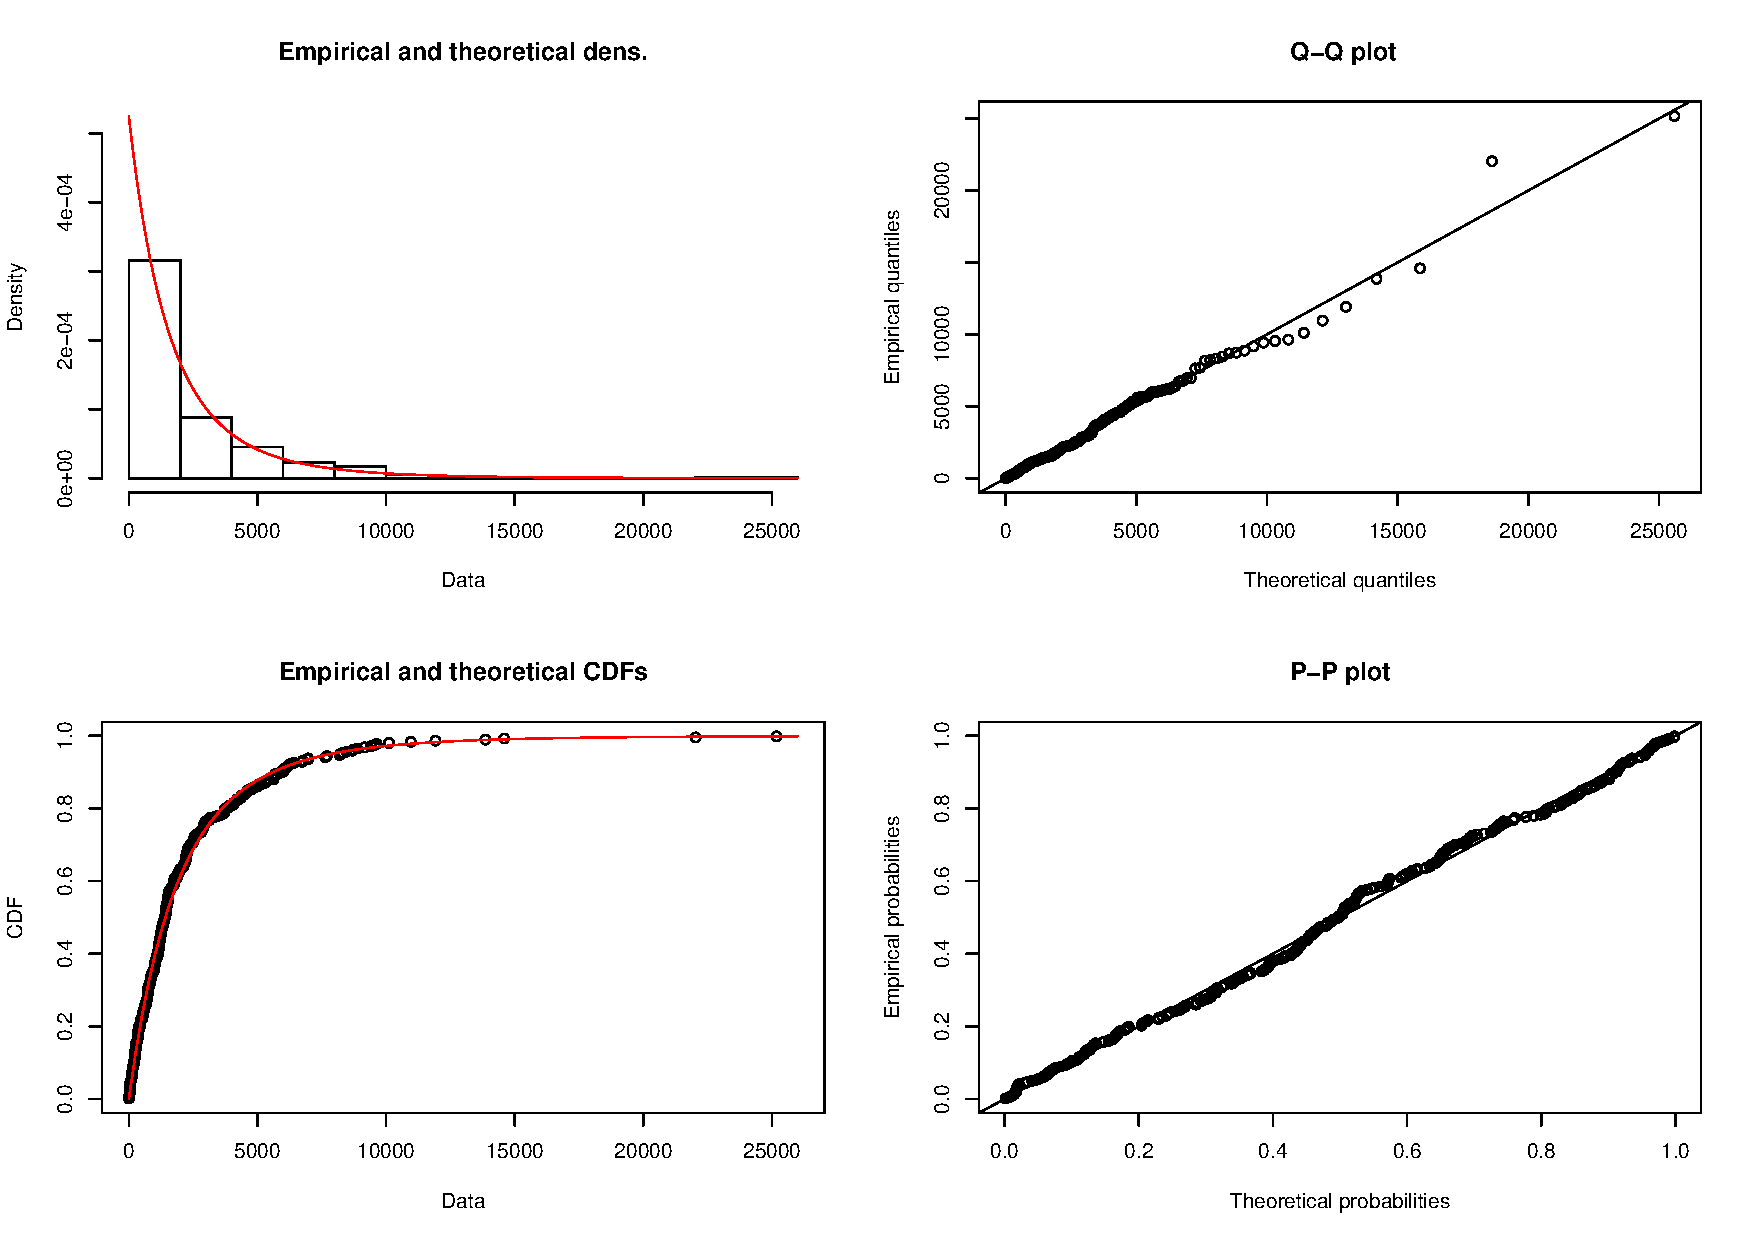
\includegraphics[width=18cm, height=10.5cm]{inter_arrival_pareto.pdf} 
\caption{Density, CDF, P-P and Q-Q plots for a fitted Pareto Distribution against inter-arrival time data}
\end{center}
\label{fig:outagedistribution}
\end{figure*}

Table 2 shows a summary of the seven distributions fitted against the observed inter-arrival time data. Each distribution is listed along with it's corresponding Anderson Darling test statistic and p-value. Fig 1 shows four Goodness-of-fit plots for a fitted Pareto distribution: Density, Cumulative Distribution Function (CDF) , Probability (P-P) \cite{gibbons2011nonparametric}  and Quantile (Q-Q) \cite{wilk1968probability}.  

\subsection{Service time distribution}

\begin {table}
\caption {Service time distributions :  Goodness of fit summary} 
\begin{center}
\begin{tabular}{p{2.1cm} |  p{3.1cm} | p{1.3cm}} \hline \bf{Distribution} & \bf{AD Test Statistic} & \bf{p-value}
\\ \hline lognormal & 0.34 & 0.90
\\ loglogistic & 0.74 & 0.53
\\ Pareto & 1.60 & 0.15 
\\ weibull  & 6.82 & 4.00e-04 
\\ gamma & 272.44 & 1.83e-06	
\\ exponential & Infinity & 1.83e-06
\\ logistic & Infinity  & 1.83e-06	
\\ \hline
\end{tabular}
\end{center}
\end{table}

\begin{figure*}[]
\begin{center}
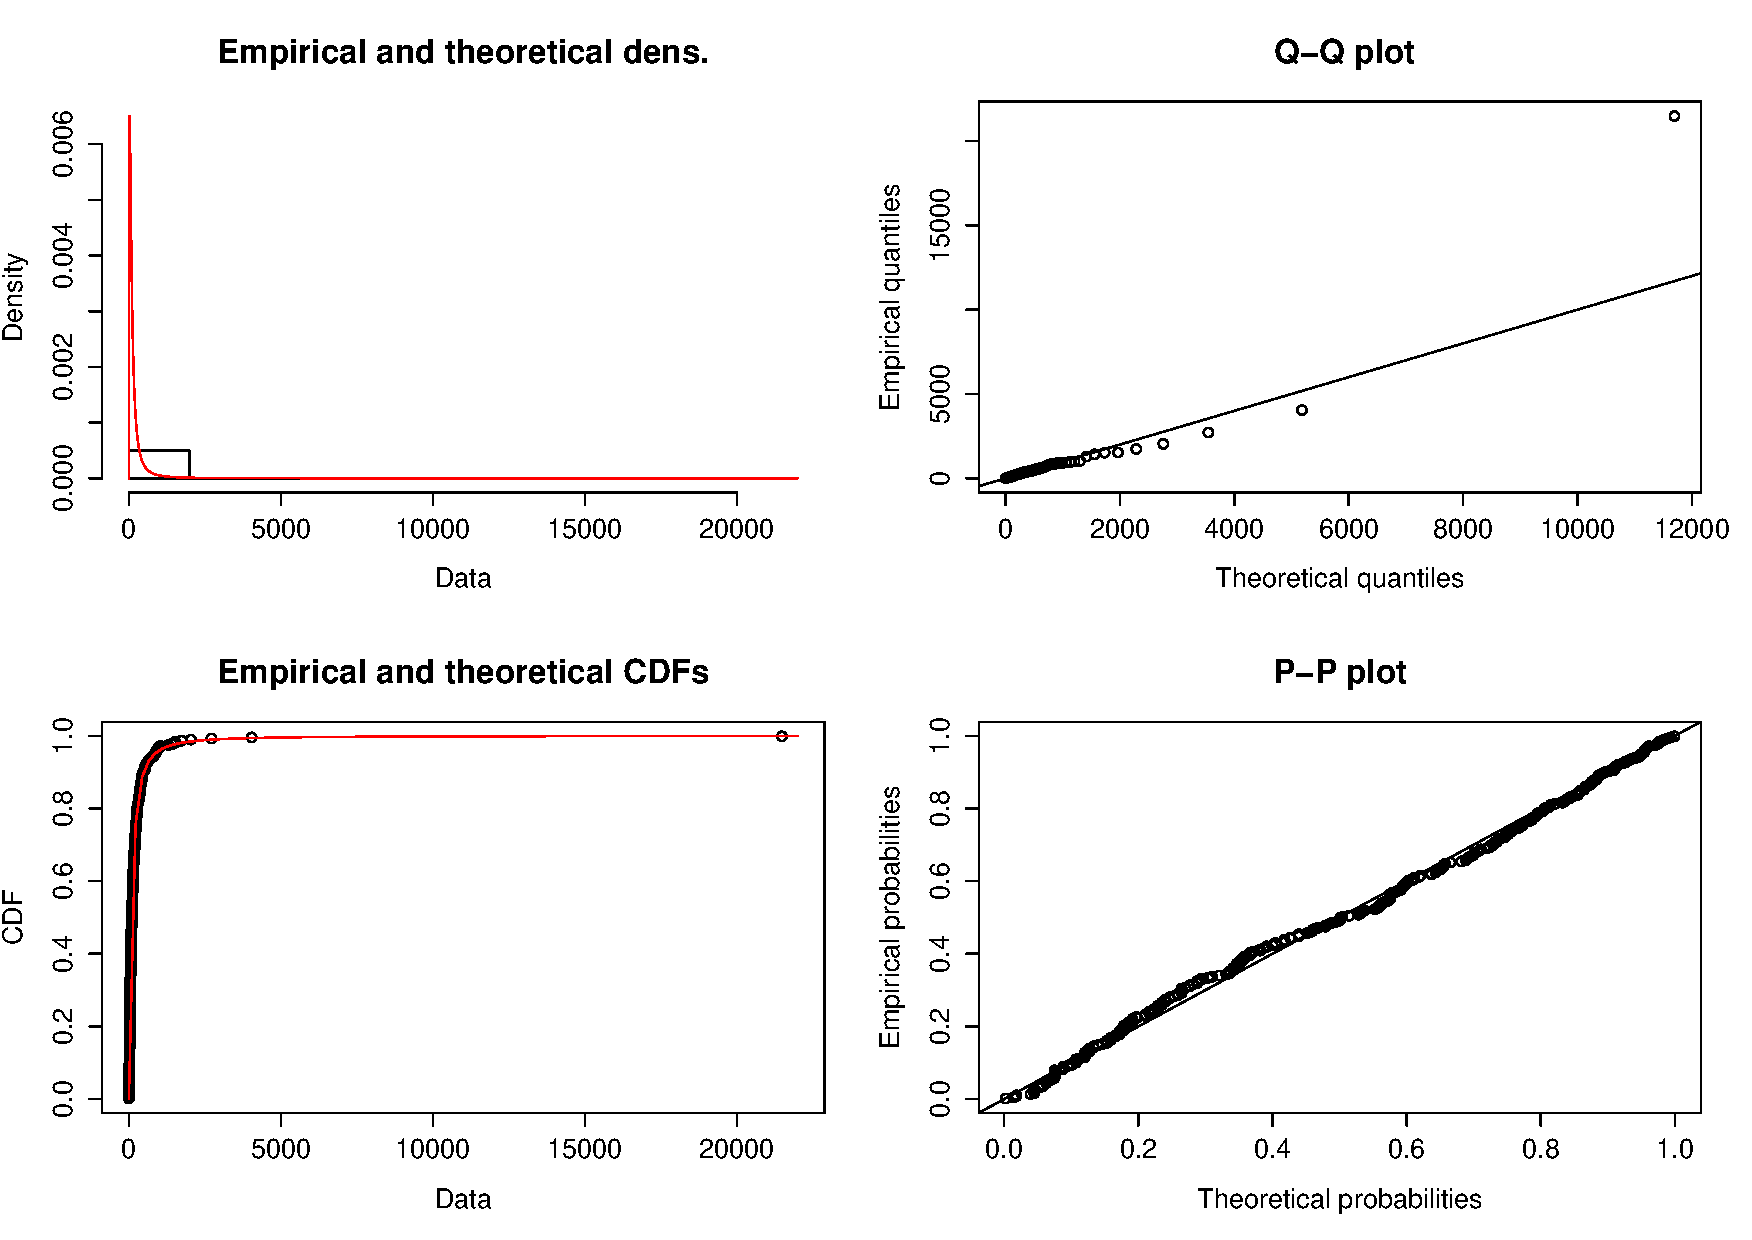
\includegraphics[width=18cm, height=10.5cm]{service_lognormal.pdf} 
\caption{Density, CDF, P-P and Q-Q plots for a fitted lognormal Distribution against service time data}
\end{center}
\label{fig:outagedistribution}
\end{figure*}


Table 3 shows a summary of the seven distributions fitted against the observed service time data. Each distribution is listed along with it's corresponding Anderson Darling test statistic and p-value. Fig 2 shows four Goodness-of-fit plots for a fitted lognormal distribution: Density, (CDF), (P-P)  and (Q-Q).  


\subsection{Outage event modelling framework}

\begin {table*}[]
\caption {Summary of queue modelling experiments and observed overlapping outage events} 
\begin{flushleft}

\begin{tabular}{l | l | l | p{10cm} l} \bf{Model Type} & \bf {\% Busy} & \bf {\% Free} & \bf {Comments} 
\\ \hline Observed Data & 7.9 &  92.1 & 331 outage events collected over an 18 month period (Jan'15 - Jun'16). 26 outage events had overlapping inter-arrival and services. In other words 26 outage events arrived while an existing outage was being serviced. 

\\  Simulation (G/G/1) & 6.2 &  93.8 &  The queue model was composed of a Pareto and lognormal distribution for inter-arrival and service times respectively. The simulation was executed 1M times to ensure a sufficient number of data points.

\\  Simulation (M/M/1) & 3.0  &  97.0 &  The queue model was composed of a Poisson process and exponential distribution for inter-arrival and service times respectively. The simulation was executed 1M times to ensure a sufficient number of data points.
\\ \hline 

 \end{tabular}
\end{flushleft}
\end{table*}

Table 4 shows a summary of the queue model experiments conducted as well as details of the observed outage data over an eighteen month period. The model type defines whether observed data or a simulation was conducted. The type of simulation is also included. The \% Busy and \% Free columns relate to the number of overlapping events in the queue. For example we count the number of times an outage event (either observed or simulated) entered the queue system while an existing outage was currently being serviced. This value is presented as an overall percentage. Finally the comments column provides some additional details as to the number of events that were used as part of the overall busy and free calculation along with the type of distribution that was used as part of the queue simulation experiments. 

\subsection{Assessment for no association and linkage between overlapping outage events}

Analysis of the inter-arrival times between outages showed that 26 outages overlapped with existing outage events. For each of these 26 overlapping outages, the authors inspected each outage report to determine if their was a link between these outages and outages already in the queue. The authors looked at the component affected and the root cause to determine whether a link between events was present.The authors looked at both the overlapping outage and the current serviced outage to determine this link. Table 5 shows a summary of this work.


\begin {table*}[]
\caption {Summary details of overlapping outages with analysis of component area, root cause and linkage assessment} 
\begin{flushleft}

\begin{tabular}{l | l | l | p{9cm} l} \bf{Outage} \# & \bf{Component} & \bf{Root Cause} & \bf{Outage Details} 
\\ \hline  1 & E-mail &  Network & Cascade network failures were observed in the email component.  A second network failure was observed due to latency caused by the first network failure. Assessment: Outages linked.
\\ \hline 2 & E-mail  & Network & A network bottleneck was observed. A configuration change was made to alleviate the bottleneck, this change caused additional bottlenecks. Assessment: Outages linked.
\\ \hline 3 & E-mail  & Concurrency &  A failover operation failed to work correctly which caused an outage, while the system was in a failed state, crash log information was not output correctly. Assessment: Outages linked.
\\ \hline 4 & Social & High Availability & A number of nodes in the social component failed due to a server crash. While these nodes were down, extra load was added to the available nodes in the cluster which caused a subsequent outage. Assessment: Outages linked.
\\ \hline 5 & E-mail & Network & A temporal network outage occurred in the E-Mail system. Most of the nodes failed gracefully and returned to normal operations, however a number nodes did not fail gracefully which caused a secondary outage. Assessment: Outages linked.
\\ \hline 6 & E-mail & Configuration & A service on the E-mail system failed due to contention. A config change was made to remediate. The config change caused additional contention further along the service stack. Assessment: Outages linked.
\\ \hline 7 & Collaboration & Network & A temporal network outage occurred in the collaboration component, which caused all nodes to fail gracefully, almost all nodes returned to normal when the network was restored. A number of nodes however were in a hung state (from the initial outage) which caused a secondary outage. Assessment: Outages linked.
\\ \hline 
 \end{tabular}
\end{flushleft}
\end{table*}

Table 6 shows a 2 by 2 contingency table which contains counts of overlapping, non-overlapping, linked and non-linked outages. The null hypothesis states there is no association between overlapping outages and linked between prior outages. Fishers exact test was used for the no association test. A p-value of \textless 0.001 was calculated. 

\begin {table}
\caption {Test for no association between overlapping and linked outages using Fisher's exact test} 
\begin{center}
\begin{tabular}{p{2.7cm} |  p{1.1cm} | p{2cm}} \hline \bf{Outage type} & \bf{Linked}  & \bf{Non-linked}
\\ \hline Non-Overlapping  & 0 & 305
\\ Overlapping & 7 & 19
\\ \hline
\end{tabular}
\end{center}
\end{table}

\section{Discussion}

Section 4 presented the results of distribution fitting, queue modelling and test for no association between overlapping outage events. The following section provides deeper analysis and discussion of these results.

\subsection{Inter-arrival time distribution}

\subsection{Service time distribution}

\subsection{Outage event modelling framework}

\subsection{Assessment for no association and linkage between overlapping outage events}

\section{Conclusion}

Our conclusion starts here........

\section{Future work - SHOULD THIS MOVE TO DATA SET AND METHODOLOGY}

By using the simple queue as a starting point, future work is planned to validate the framework in the context of a complex queuing system (i.e. a queue with multiple "servers"). John \cite{john1963single} discusses dependencies between inter-arrival and services times within a queue system as the assumption of independence between the two times are not always valid. \par Future work will also include research into the relationship between inter-arrival and service time durations and how these durations relate to service level agreement impact.



\section*{References}

\bibliography{journal-bib}

\end{document}